\mysubsection{Message et communication asynchrone}

\ifbook{
  \mysubsubsection{Problématique de la communication asynchrone}
    \paragraph{} Depuis les débuts de l'informatique, le besoin d'une communication \textbf{asynchrone} entre
    deux processus ou deux programmes est présent et les problématiques liées à ce genre de communication sont
    bien connues. Tout langage de programmation fournit les primitives nécessaires à l'implémentation d'une telle
    communication, mais on fait désormais plus souvent appel à des \textit{middlewares} dédié. Ainsi, le
    monde du \textit{Message Oriented Middleware} a émergé, autant pour faciliter le développement qu'assurer une
    bonne gestion des messages échangés.
}

\ifslide{
  \begin{frame}{Problématique de la communication asynchrone (1/2)}
    \begin{block}{Motivations}
      \begin{itemize}
        \item \textit{fire and forget}
        \item \textit{can't wait}
        \item \textit{producteur / consommateur}
      \end{itemize}
    \end{block}
  \end{frame}
}

\ifbook{
 \paragraph{} Avant d'avancer plus en avant dans la description du fonctionnement générale de ces
 \textit{middlewares} étudions rapidement les cas d'utilisation qui motivent leurs utilisations.
 Sans être exhaustive, voici quelques exemples, volontairement très générique, de cas d'utilisation
 où l'on souhaite généralement mettre en place une communication \textbf{asynchrone} entre deux
 processus:

 \begin{description}
   \item [\textit{"fire and forget"}] Un processus souhaite communiquer une information à un autre,
   sans attendre que ce dernier est fini son traitement pour continuer (ex: journalisation des
   opérations d'une application). Généralement, dans ce genre de cas, le traitement qui doit être
   réalisé par le second processus n'a pas d'impact sur celui réalisé par le premier, qui peut donc
   continuer sans attendre.
   \item [producteur et consommateur] Problème d'algorithmique classique, le
   \mylink{http://fr.wikipedia.org/wiki/Mod\%C3\%A8le\_producteur-consommateur}{modèle
   producteur/consommateur} est un cas d'étude classique d'une communication asynchrone. En
   quelques mots, le processus producteur dépose, dès qu'il peut, une demande de traitement dans une
   sorte de "boite à message", qu'un processus consommateur, quand il le souhaitera ou pourra,
   récupérer, et effectuer le traitement nécessaire.
 \end{description}
}


\ifslide{

  \begin{frame}{Problématique de la communication asynchrone (2/2)}
    \begin{block}{Problématiques}
      \begin{itemize}
        \item gestion d'erreur
        \item gérer les queues
        \item persistance (ou non) des messages
      \end{itemize}
    \end{block}
  \end{frame}
}

\ifbook{

  \paragraph{} La nature même de la communication induit rapidement le besoin de gérer l'état des
  messages échangés. En effet, à partir du moment où la réception d'un message n'est pas immédiate,
  il va souvent devenir nécessaire de s'assurer que ces derniers soit persistés et administrer. Il
  s'agit d'un point est un important, car si les messages ne sont jamais consommés par exemple, le
  système peut rapidement se retrouver dans un état instable, car débordé de message qui ne
  "disparaissent jamais"...

  \paragraph{} Il devient rapidement nécessaire de gérer donc des files d'attentes (\textit{Queues} en
  anglais) ainsi que des erreurs de transmission. Au regard de ces quelques points, il apparait
  clairement que tout ceci offre là encore, un terrain d'investigation intéressant pour la conception
  de \textit{middleware}...
}

\ifslide{

  \begin{frame}{Message Oriented Middleware (MOM)}
    \begin{block}{Domaines}
      \begin{itemize}
        \item Publish/Subscribe (pub/sub) : n producteurs, n consommateurs
        \item Point To Point (PTP) : n producteurs, 1 consommateur
      \end{itemize}
    \end{block}

    \begin{center}
      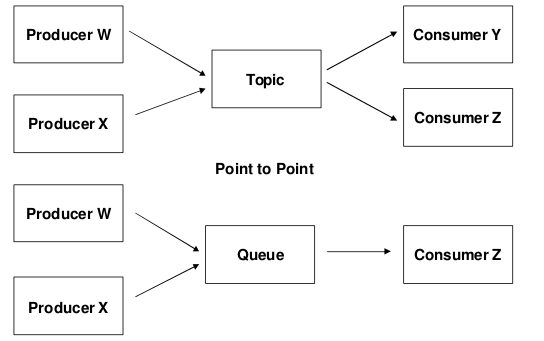
\includegraphics[scale=0.3]{img/topic-queue.png}
    \end{center}
  \end{frame}
}

\ifbook{

 \paragraph{} Un autre avantage des \textit{MOM} (\textit{Message Oriented Middleware}) est aussi la
 capacité d'effectuer une communication de 1 à n tiers aisément. En effet, une fois un message remis
 à tel programme, ce dernier peut le mettre à disposition d'un ou plusieurs processus. Ainsi, on
 peut disposer de plusieurs processus (ou même machine) prête à consommer les messages transmis.

 \mysubsubsection{Un exemple de standardisation des MOM : Java Message Service}

 \paragraph{} Sans rentrer dans les détails de cette API Java\footnote{Voir
 \mylink{http://en.wikipedia.org/wiki/Java_Message_Service}{Java Message Service}}, nous
 pouvons juste retenir que, reprenant la théorie évoqué plus haut, cette spécification définit
 l'API que doit supporter et respecter un MOM implémenté en Java.

 \paragraph{} En plus de fournir les services d'administration et de diffusion évoqués, cette
 API assure aussi un fort \textbf{découplage} entre le logiciel client (utilisant l'API) et
 l'implémentation de la spécification JMS qu'il utilise. Ceci permet ainsi de facilement remplacer
 une implémentation par une autre - sans altérer le comportement du programme\footnote{Bien
 évidemment, les performances, comme les limites du composant varieront selon l'implémentation
 utilisée - toute la difficulté étant donc le choix judicieux de cette dernière.}.

 \paragraph{} La figure \ref{jms-steps} présente, dans les grandes lignes, les composants logiciels
 impliqués lors d'une communication aynchrone utilisant JMS.

  \begin{center}
    \begin{figure}
      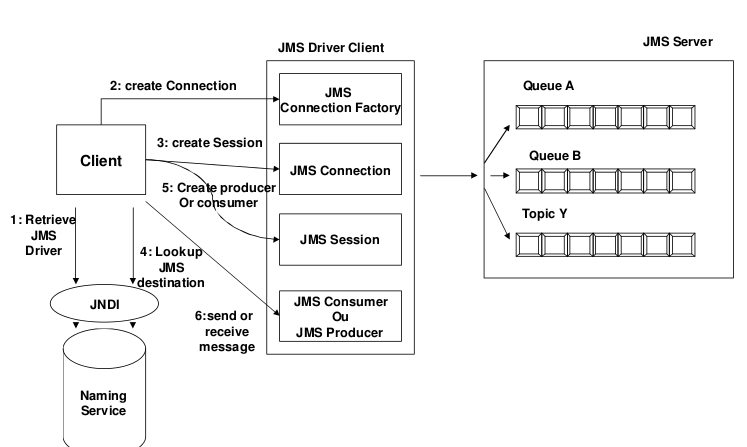
\includegraphics[scale=0.3]{img/jms-steps.png}
      \label{jms-steps}
      \caption{Vue générale d'une communication asynchrone à l'aide de JMS}
    \end{figure}
  \end{center}
}

\ifslide{

   \begin{frame}
     \begin{block}{Invocation JMS}
       \begin{itemize}
         \item Localiser le driver JMS lookup JNDI. Le driver est une connection
 factory
         \item Créer une connection JMS obtenir une connection à partir de la
 connection factory
         \item Créer une session JMS :Il s'agit d'un objet qui va servir à recevoir et
 envoyer des messages. On l'obtient à partir de la connection.
         \item Localiser la destination JMS: Il s'agit du canal sur lequel les
 messages sont emis ou recus. Normalement, c'est réglé par le
 déployeur. On obtient la destination via JNDI.
         \item Créer un producteur ou un consommateur JMS. Utilisés pour écrire
 ou lire un message. On les obtient à partir de la destination et de la
 session.
         \item Envoyer ou recevoir un message
       \end{itemize}
     \end{block}
   \end{frame}

   \begin{frame}{Message Oriented Middleware (MOM)}
     \begin{center}
       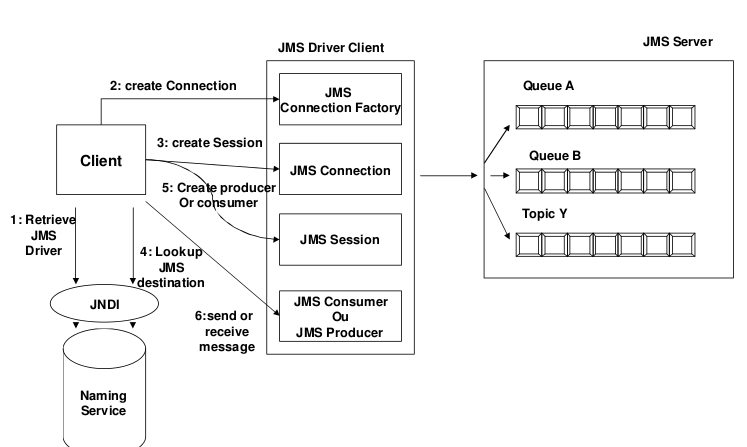
\includegraphics[scale=0.3]{img/jms-steps.png}
     \end{center}
   \end{frame}
 }

\ifbook{

  \mysubsubsection{Autre considérations relatives à l'usage des MOM}

  \paragraph{} Bien qu'en première anlayse les MOMs soient des outils relativements simple dans leur
  concept (une simple pile de message), leurs usages entrainent vite l'apparition de problématiques,
  déjà évoqués précédemment, telles que:
  \begin{description}
    \item[transactionnalité] Le MOM peut rapidement se trouver parti prenant d'échange
    transactionnel et devra donc être en mesure de supporter les contraintes qu'impliquent un tel
    contexte - spécialement si ce dernier doit prendre part à des transaction distribués (voir le
    \textit{Two Phase Commit} étudié précédemment).
    \item[sécurité] De la même manière, tous les problématiques usuels de sécurité, ainsi que les
    méchanismes classiques associés, se retrouvent lors du dépoiement d'un MOM au sein d'un
    système. Un MOM offre donc généralement des fonctionnalités d'authentification et
    d'authorisation et peut utiliser différents mécanismes (certificat, mot de passe, ...) pour les
    implémenter.
  \end{description}

}

\ifslide{

  \begin{frame}{Message Oriented Middleware (MOM)}
    \begin{block}{Domaines}
      \begin{itemize}
        \item Transactions and MBD %: La production et la consommation du message sont dans deux transactions séparées...
        \item Sécurité %: Les MDB ne reçoivent pas les informations de sécurité du producteur avec le message.
      \end{itemize}
    \end{block}
  \end{frame}
}

\ifbook{

  \mysubsubsection{Rôle d'un MOM dans l'architecture d'un système}


  \paragraph{} Disposer d'un MOM au sein de son architecture logicielle apporte de nombreux
  avantages. Premièrement, on dispose d'un mécanisme permettant d'établir, de manière indépendante
  du protocole sous jacent, une \textbf{communication par message}, dans laquel le MOM fait office
  d'intermédiaire.

  \paragraph{} Ce rôle d'intermédiaire permet au MOM d'apporter plusieurs fonctionnalités
  très intéressantes en termes de \textbf{découplage} et de stratégie de \textit{montée} ou
  \textbf{répartition} de charge. Ainsi, on peut en effet imaginer, par exemple, utiliser un MOM
  pour faire office de tampon temporaire entre deux systèmes, pour adapter une différence de
  fréquence entre le système producteur de message, très rapide, et celui ou ceux qui les consomment
  et traitent, vraisemblablement plus lent.

  \paragraph{} Un autre exemple est le \textbf{routage de message}. Une application se contente d'envoyer des
  messages à un MOM, et celui ci redistribue les messages, selon leur métadonnées, à différents
  systèmes consommateurs. Bien évidemment, on peut aussi placer plusieurs instances du MOM en parallèle et
  effectuer, entre ces différentes instances, un équilibrage de charge.

  \paragraph{} Tout ces exemples soulignent bien la souplesse et la flexibilité qu'un MOM peut
  donner à une architecture logicielle. Ces derniers accroissent nettement la complexité d'un
  système.
}

\ifslide{
  \begin{frame}
    \begin{block}{Advantages}
      \begin{itemize}
        \item message-based communications protocol
        \item store/buffer
        \item routing / load balancing
      \end{itemize}
    \end{block}
  \end{frame}

  \begin{frame}{Standardisation ?}
    \begin{block}{No Standard yet :( (API only) }
      \begin{itemize}
        \item JMS (Java Messaging System)
        \item MSMQ (Microsoft Message Queuing)
        \item Amazon Simple Queue Service
      \end{itemize}
    \end{block}

    \begin{block}{Protocol}
      \begin{itemize}
        \item AMQP (Advanced Message Queuing Protocol) - protocole
        \item STOMP (Streaming Text Oriented Messaging Protocol)
      \end{itemize}
    \end{block}
 \end{frame}

 \demoframe{Communication Asynchrone}{Exemple avec JMS}
}
